\chapter{Introduction}

\section{Motivation}
Current data sets are often generated through extensive experiments utilizing full-scale systems such as MilliAmpere.
While these experiments are necessary for specific research purposes, the cost-benefit ratio may not be proportional when the primary goal is collecting sensor data.

Recognizing the challenge at hand, I embarked on the development of human operable \sr during my preproject.
The objective was to develop a lightweight \sr that addressed common challenges such as synchronization and pose estimation, paving the way for a low threshold approach to high quality data acquisition.

While most of the hardware and electronics were completed during the preproject, much remained including the challenge of developing a software stack that can effectively manage the large amount of custom raw data produced by the two polarization cameras.




The motivation behind this project stems from my pursuit of an integrated Ph.D.
program, where I will focus on investigating the potential enhancements in detection capabilities for Autonomous Surface Vessels (ASVs) through the integration of data from various sensors, such as lidars and specialized cameras.
This research will heavily involve machine learning techniques, necessitating a significant amount of training data.
Since I will be exploring new sensor combinations, existing datasets alone cannot fulfill the requirements.
Hence, there is a need for a framework that enables the collection of new data, with a preference for a low threshold approach.
Therefore, the development of this sensor rig becomes imperative.


\begin{figure}
    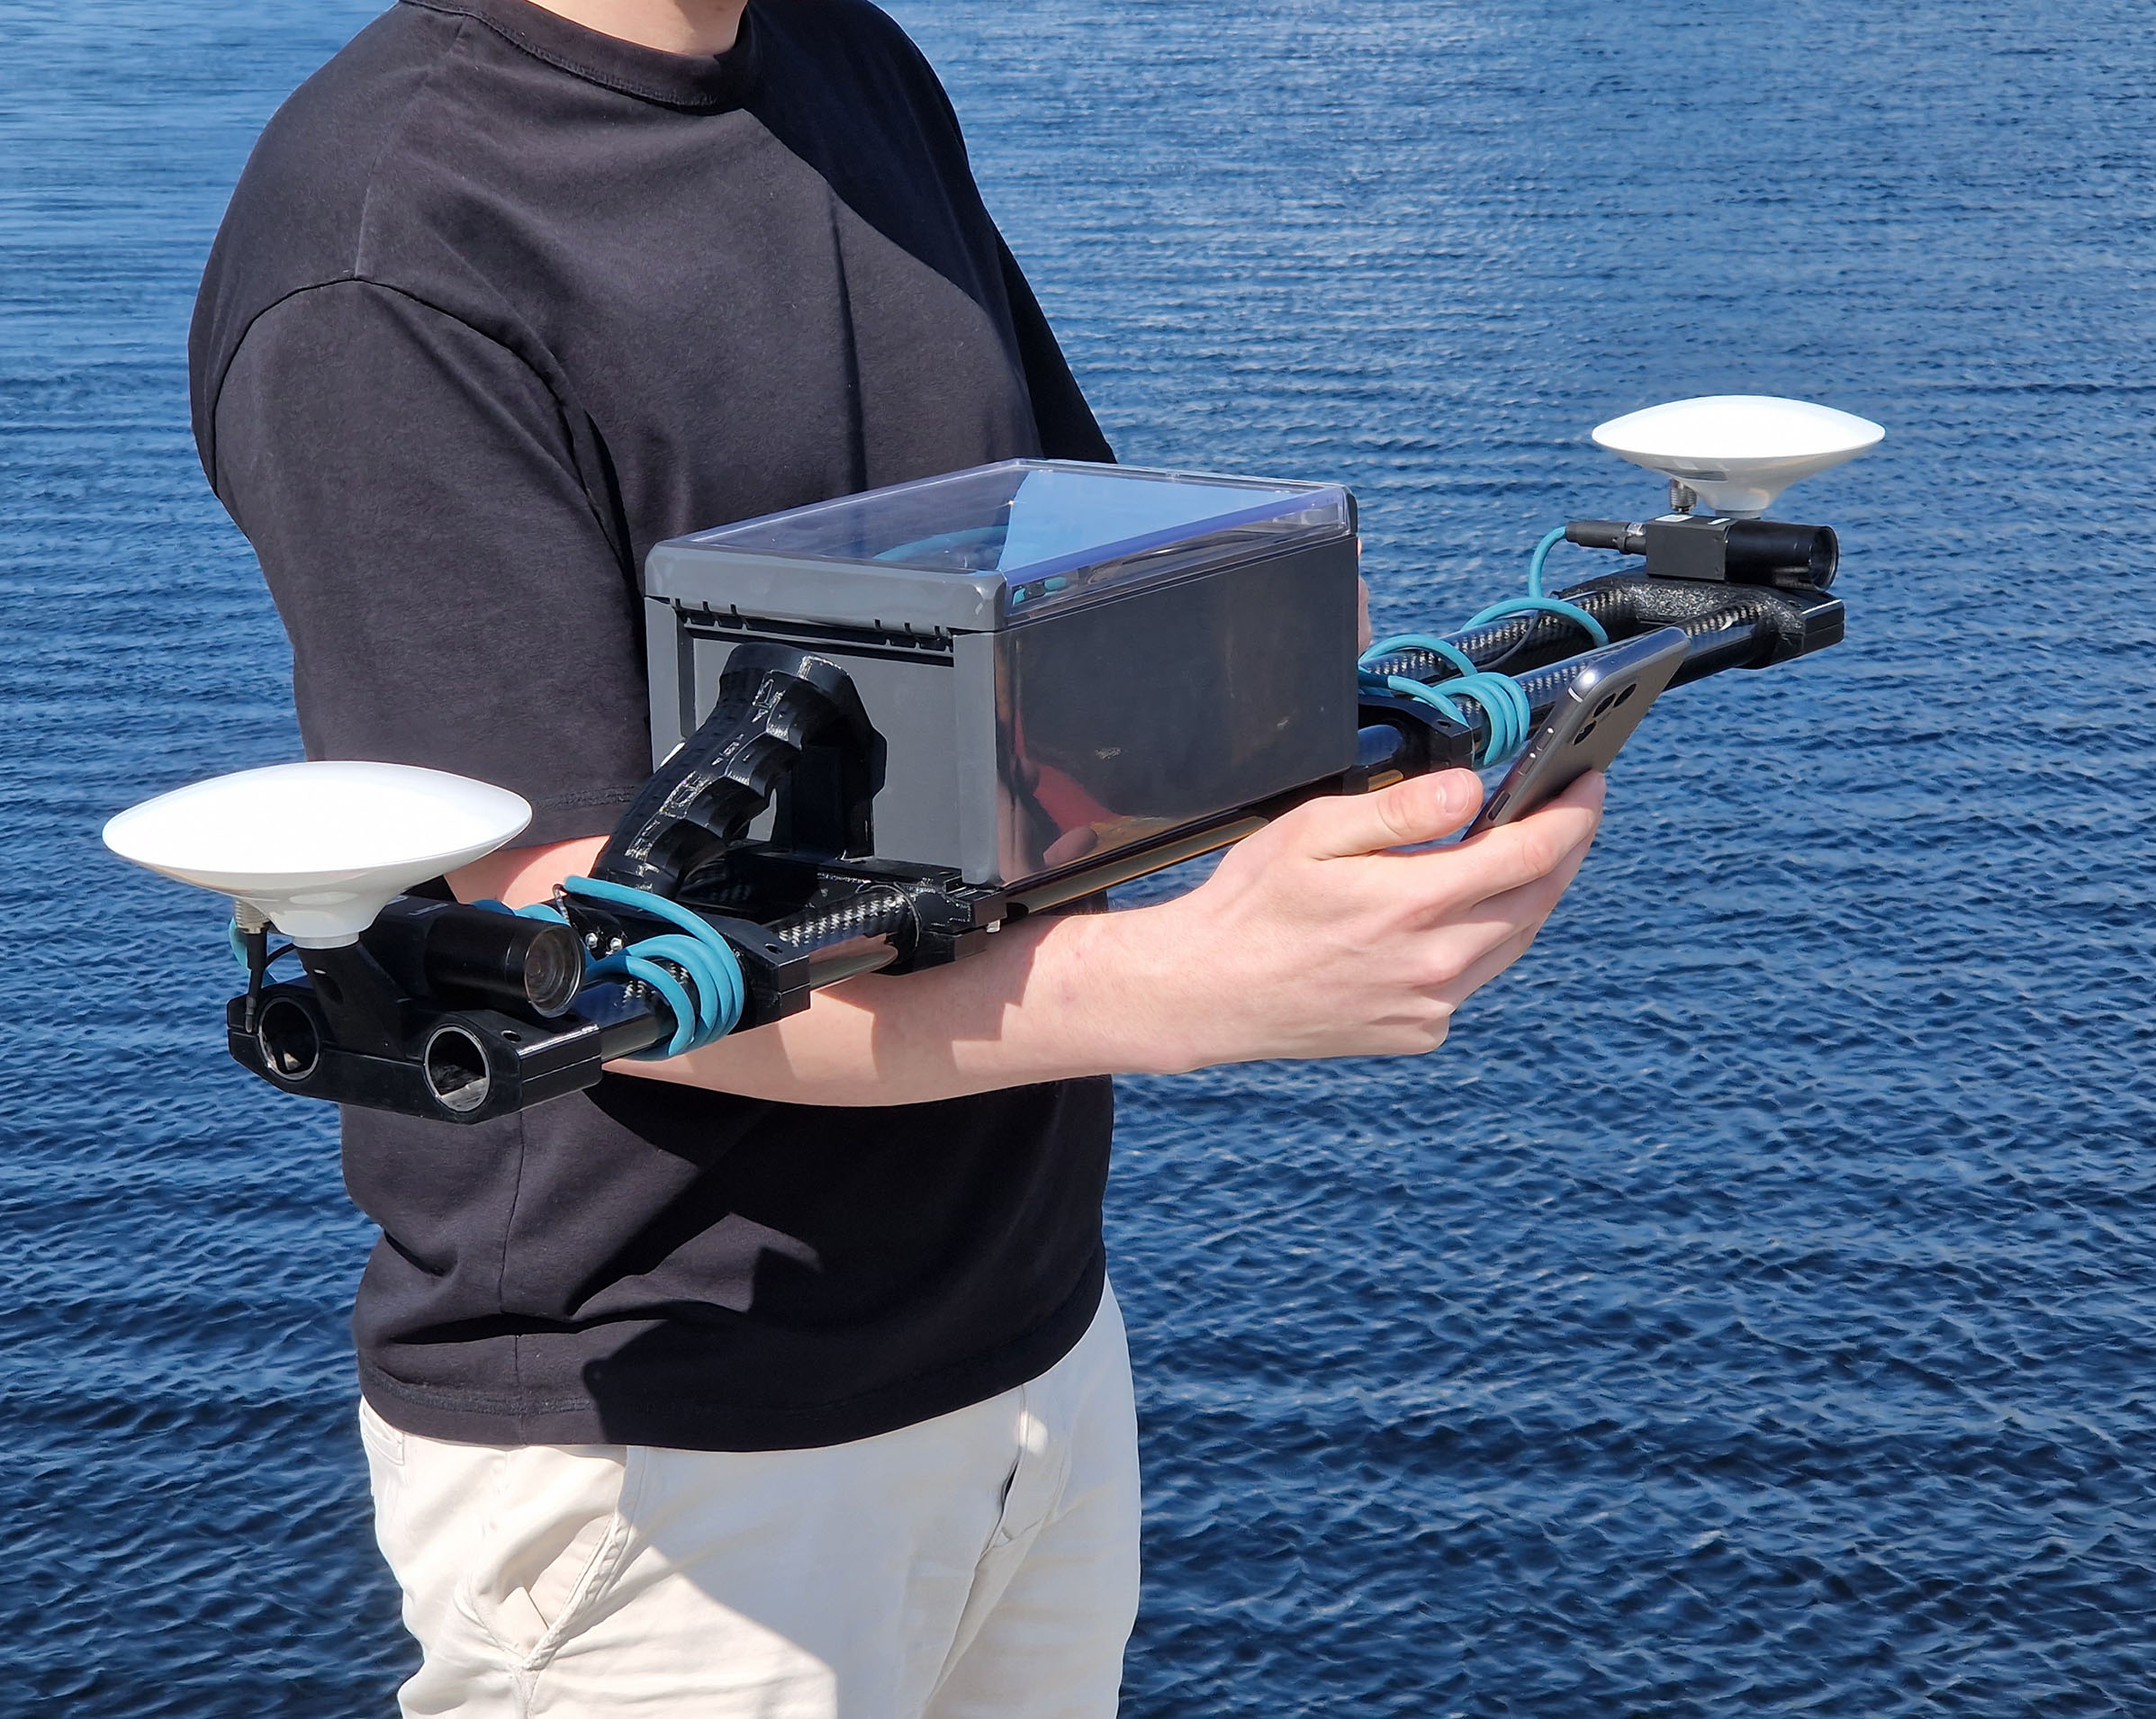
\includegraphics[width=\textwidth]{figures/frontpage.jpg}
    \caption{The Sensor Rig}
\end{figure}
\section{TODO}
Explain how this project is a bit all over the place but show how it ties together with a full page figure.


\section{Motivation}
A significant amout of work was put into enabling on the fly compression of the videostreams from the \sr.
That is the ability to compress the video data as it is being recorded, and storing the compressed data on disk.

The cameras on the \sr produce roughly $2Gb/s$ of data.
Aditionally, the \gls{imu} and \gls{gnss} produce data, but amount is neglible compared with the cameras.
At this rate it infeasable to record long datasets as almost a terrabyte of data is produced every hour.
\begin{align}
    \frac{1TB}{2Gb/s}  = \frac{8Tb}{2Gb/s} = 4000s \approx 1h + 7min
\end{align}

It is reasonable to say that a much easer option is to buy \gls{ssd} with a capacity up to 8TB \cite{CorsairMP600PRO}, enabling roughly 9 hours of recording.
One reason this
\cite{microntechnologyMicron2300SSD2020}


\subsection{Limited write speed}
One issue when storing the raw data at first was that the \jx was not able to write to the disk fast to the installed \gls{ssd}.
The write speed was tested using:
\begin{minted}[linenos=false]{bash}
    sudo dd if=/dev/zero of=./testfile bs=8k count=100k conv=fdatasync
\end{minted}
which repeatedly reported write speeds just below $2Gb/s$ (250MB).
This is weird, as the \gls{ssd} has a write speed of $2.7GB/s$, but other people have faced similar issues on the \jx \cite{microntechnologyMicron2300SSD2020} \cite{dtyuImbalancedPerformanceRead2018}.
This is probably fixable, but provides further motivation to enable on the fly compression


\subsection{Integration with other systems}
The main intended purpose of the \sr is to be carried around by a human operator and

\subsection{Streaming to external devices}
Having a


\section{Challenges}
The main challenge in this project has been to design a system that can effectively manage the large amount of raw data produced by the two cameras.
Each camera features a 5.0MP sensor configured to capture 10-bit raw images 16 times every second \cite{lucidvisionlabsTriton0MPPolarization}.
To put this into perspective, a single frame contains more data than what is needed to store the entire collection of William Shakespeare's works in plain text \cite{projectgutenbergCompleteWorksWilliam1994}.

If the output from these cameras were stored directly to disk, almost a Terabyte of data would be generated every hour, making it infeasible to collect long term data sets.


\section{Outline}
Creating the \sr has been a large undertaking and I have worked on wide variety of different topics including ergonomic hardware design, full stack web development, kernel compilation and low level optimizations in CUDA.
The only thing that is consistent between all the different parts is that they are performed in order to acheive the goal of creating a human operable soensor rig for high quality data collection.










The first, and most extensive part is the software development requiered to collect and compress the data from the \sr in real time.
As this has been the main focus of the project and also is what is most relevant, the first five chapters are dedicated to this.
Following this

\paragraph{Chapter \ref{chap:programming_theory}: Real time programming on Jetson Xavier}
This chapter provides an overview of the theoretical background necessary to achieve real-time performance on the \jx platform.
It covers topics such as real-time programming theory, performance considerations for heterogeneous systems, and a brief introduction to the CUDA programming model.

\paragraph{Chapter \ref{chap:cameras}: Polarization Cameras}
This chapter explains how interaction with the camera is acheived, how they are configured and how various the network adapters have been configured to acheive $2Gb/s$ throughput from the \cams.

\paragraph{Chapter \ref{chap:debayer}: Efficient processing of raw image bitstream in CUDA}
To make it possible to compress the video streams, the raw data has to be transformed into a format that can be processed by the \gls{h265} encoder.
This chapter explains how this is acheived in real time using CUDA.

\paragraph{Chapter \ref{chap:gstreamer}: Video Compression using GStreamer}
\gls{gstreamer} is a powerful framework for processing video streams.
This chapter explains how it is used to compress the video streams in real time using hardware accelration on the \jx.

\paragraph{Chapter \ref{chap:pipeline}: Pipeline Assembly in Python}
\todo

\subsection{Web interface for control and monitoring}

\paragraph{Chapter \ref{chap:gui}: Web Interface to Control, Monitor and Stream Video}
A web application was developed to enabling real time control and monitoring of the \sr and its video streams.
This allows anyone with a smartphone to operate the \sr without any prior training or technical knowledge.


\paragraph{Chapter \ref{chap:flashing_xavier}: Compiling Jetson Linux with PPS}
In order to get the the \gls{gstreamer} pipeline working, it was necessary to update the operating system to a newer version.
As a \gls{pps} signal is used to synchronize the clock on the \jx to \gls{utc}, it was necessary to compile the kernel with support for this, which turned out to be a non-trivial task demanding a systematic approach.

\paragraph{Chapter \ref{chap:hardware}: Improving the Hardware}
After the \preproject most of the hardware was already in place, but some parts were missing.
I applied for, and got, funding to purchase a new 3D printer to enable an iterateive design process.
With this in place custom ergonomic carry handles, new combined camera and antenna mounts and other minor parts were designed and 3D-printed.

\paragraph{Chapter \ref{chap:results}: Results}


\paragraph{Chapter \ref{chap:future_work}: Ongoing developments and future work}
Some design flaws from the \preproject remain to be fixed and a few possible performance improvements have been identified.
With the goal of creating a fully autonomous sensor rig acheived, the next step is to create state of the art stereo polarization datasets and advance the field of situational awareness for autonomous surface vessels.


\section{Contributions}
Automated pipeline for compiling and flashing Jetson products.
High performance custom debayer algorithm for Polarization RGS cameras written in CUDA.
Development and manufacturing of ergonomic carry handles.
Software pipeling for real time image debayering and compression built on GStreamer.
Framework for creating real time graphical web interfaces.

\section{Proof of }
